\subsection{Fight model}\label{chap:fightDef}
We define the \textit{state space} as the set of all possible values remaining hitpoints can have during a fight. For a fight against an enemy with $h$ maximum hitpoints the state space is $\{0,\ldots,h\}$. Let $H_k$ be the number of hitpoints the enemy has remaining after $k$ hits. Fights can be labeled with a sequence of hitpoint states $(H_k)_{k=0}^{n}$ visited during the fight. For this to make sense we must have $H_n=0$ (fight ends in death) and $h \geq H_k > 0$ for $k<n$ (death does not happen before the last hit).
The probability of transitioning to state $i$ from state $j$ is called the \textit{transition probability} and is defined as
\begin{align}\label{eq:transitionProbabilities}
    p_{ij} = \Pr{H_k = i \mid H_{k-1} = j}.
\end{align}

Let $\mathcal{S}_j^n$ be the set of all possible $n$-hit fights against an enemy with $j$ hitpoints remaining. The simplest possible case are the 1-hit fights $\mathcal{S}_j^1 = \{(j,0)\}$. The sets of all longer fights can be defined recursively by noticing that if the first hit lowers the hitpoints to $i$, the remaining sequence of states is equivalent to a fight of length $n-1$ against an enemy with $i$ hitpoints remaining. In other words
\begin{align}
	\mathcal{S}_j^n &=  \{j\} \times \bigcup_{i=1}^h \mathcal{S}_i^{n-1} \quad \mbox{for } n>1.\label{eq:fightRecursion}
\end{align}
For the set of all 2-hit fights this gives $\mathcal{S}_j^2 = \{(j,h,0), (j,h-1,0), \ldots, (j,2,0), (j,1,0)\}$.

\begin{figure}[h]\label{fig:randomWalk}
    \centering
    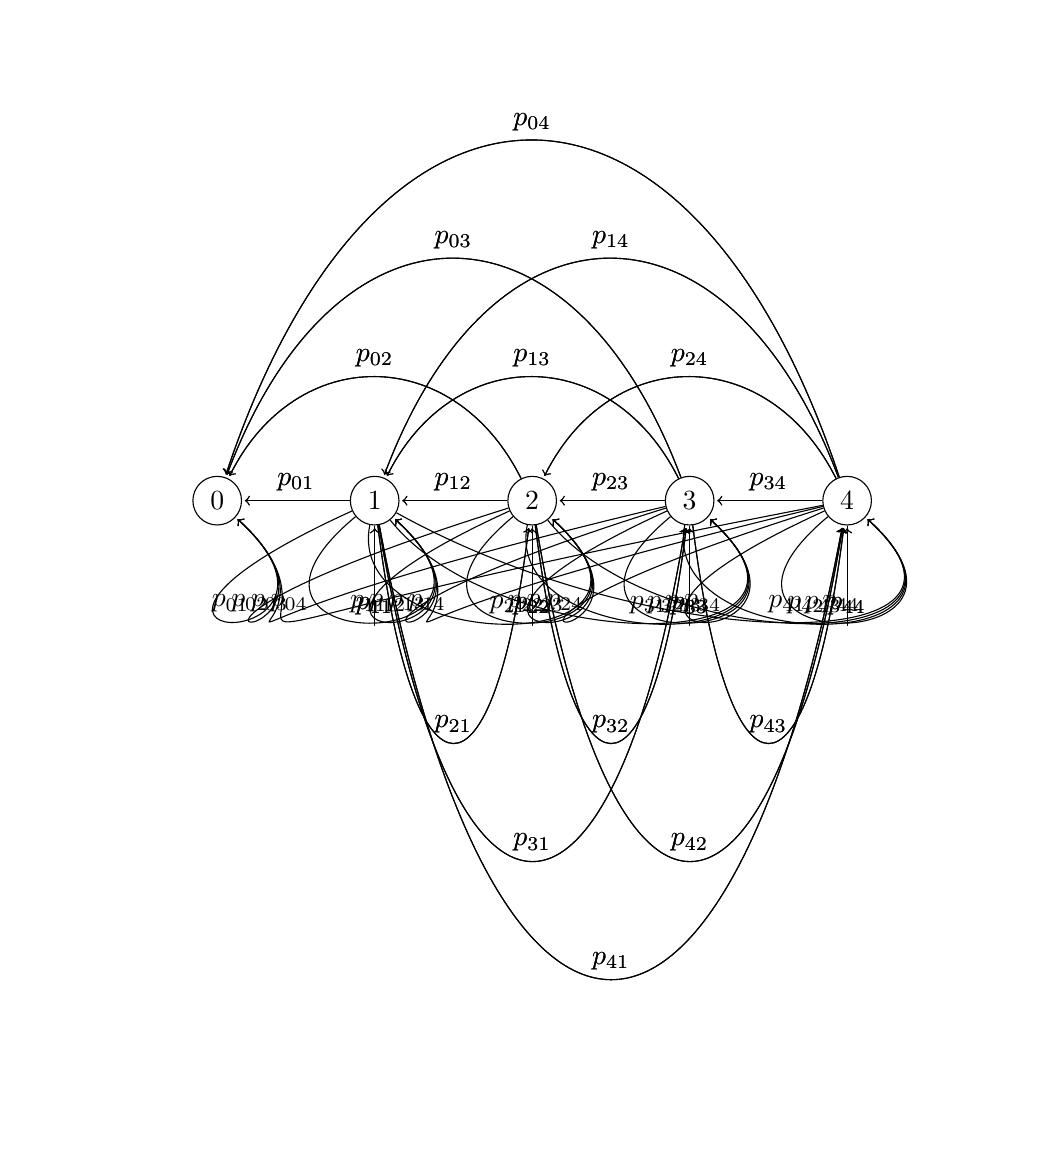
\begin{tikzpicture}[shorten >=1pt,node distance=1cm]
        \tikzstyle{state}=[shape=circle,draw,minimum size=1cm];
        \coordinate (n0);
        \xdef\scale{2}
        \xdef\maxhit{3}
        \foreach \s in {0,1,2,3,4} {
            \node[shape=circle,draw](n\s) at (\scale*\s,0){$\s$};
        }
        \foreach \from in {1,2,3,4} {
            \foreach \to in {0,1,2,3,4} {
                \foreach \y [evaluate=\y as \yeval using \from-\to] in {1} {
                \foreach \m [evaluate=\m as \meval using int(\to+\maxhit+1)] in {1} {
                    \ifthenelse{\from>\to \AND \from<\meval \AND \to>0}{
                        \path[draw,->] (n\from) ..
                        controls({(0.75*\from+0.25*\to)*\scale},{2*(\from-\to-1)}) and ({(0.25*\from+0.75*\to)*\scale},{2*(\from-\to-1)})
                        .. node[above]{$p_{\to\from}$} (n\to);
                    }{}
                    \ifthenelse{\to=0 \AND \from<\meval}{
                        \path[draw,->] (n\from) ..
                        controls({(0.75*\from+0.25*\to)*\scale},{2*(\from-\to-1)}) and ({(0.25*\from+0.75*\to)*\scale},{2*(\from-\to-1)})
                        .. node[above]{$p_{\to\from}$} (n\to);
                    }{}
                    \ifthenelse{\from=\to}{
                        \path[draw,->] (n\from) ..
                        controls({(\to-1.2)*\scale},-2) and ({(\to+1.1)*\scale},-2) .. node[above]{$p_{\to\from}$} (n\to);
                    }{}
                }
                }
            }
        }
    \end{tikzpicture}\caption{Random walk diagram for $m=3$, $h=4$ and no regeneration. The probability of walking to state $i$ from state $j$ is given with the transition probability $p_{ij}$. Only edges for which $p_{ij} > 0$ are shown.}
\end{figure}
